\section{Fizyka}
\subsection{Zasady dynamiki Newtona}

Przyspieszenie bil, a co za tym idzie opis wektorowy trajektorii bil jest oparty na zasadach 
dynamiki Newtona, zgodnie z drugą zasadą:

\begin{equation}
\vec a = \frac{\vec F}{m}
\end{equation}

\subsection{Zasada zachowania pędu i energii}

Bile zasymulowane są zgodnie z zasadą zachowania pędu:

\begin{equation}
\vec p = \vec v {m}
\end{equation}

\subsection{Kolizje}

\begin{figure}[h]
  \centering
  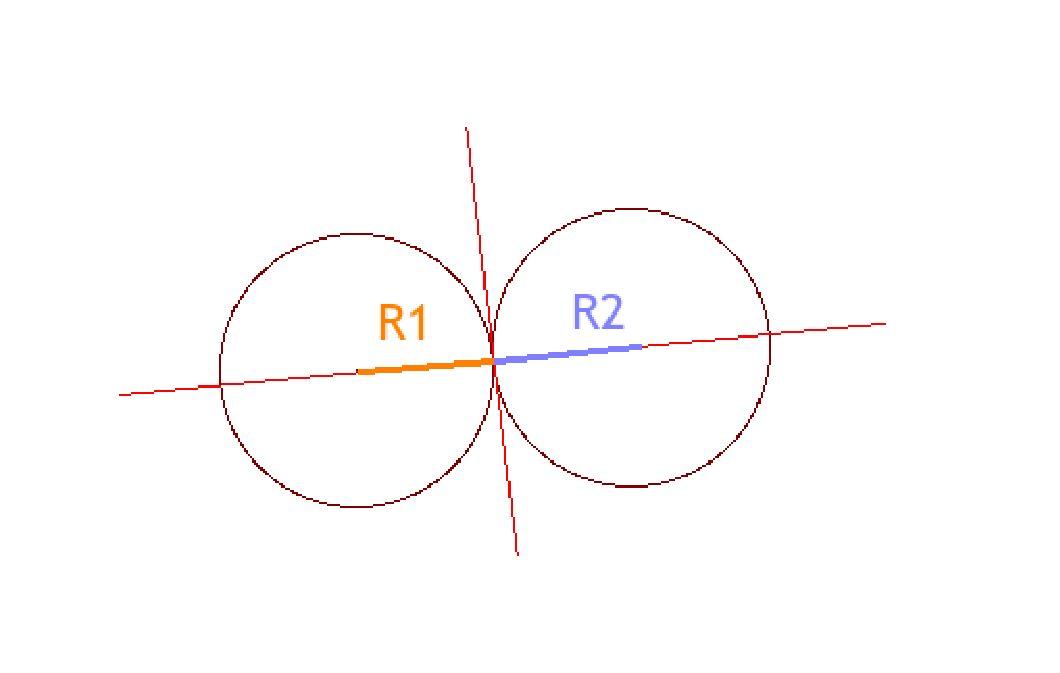
\includegraphics[width=0.5\textwidth]{./img/bb_col.eps}
  \caption{Kolizja bila - bila}
  \label{fig:bbcol}
\end{figure}

Kolizje obliczne są w możliwie najprostszy i najszybszy sposób. W naszej symulacji mamy dwa rodzaje kolizji:
\begin{itemize}
 \item bila - bila
 \item bila - banda
\end{itemize}

\begin{figure}[h]
  \centering
  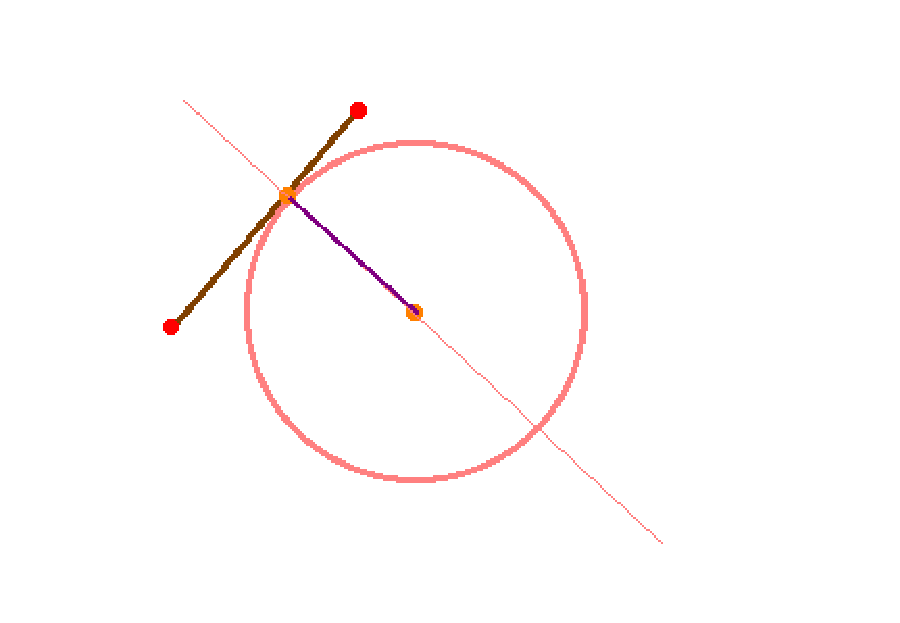
\includegraphics[width=0.5\textwidth]{./img/bbd_col.eps}
  \caption{Kolizja bila - banda}
  \label{fig:bbdcol}
\end{figure}

Pierwszy z testów kolizji polega na sprawdzeniu odległości od środków dwóch bil. Jeżeli jest mniejszy lub równy od sumy promieni bil kolizja nastapiła.\\
Drugi test jest nieco bardziej skomplikowany, bo nie można traktować testu pomiędzy bandą a bilą jako odległości okręgu od prostej, gdyż banda jest odcinkiem. Aby dobrze rozpoznać kolizję musimy dpowiednio:

\begin{itemize}
 \item sprawdzić odległość bili od prostej wyznaczonej przez 2 punkty bandy
 \item sprawdzić odległość od punktów brzegowych bandy
 \item sprawdzić czy bila znajduje się ``wewnątrz'' punktów krańcowych bandy.
\end{itemize}

Dopiero po uwzględnieniu wszystkich punktów jesteśmy w stanie jednoznacznie stwierdzić czy kolizja z bandą miała miejsce.
Tak więc system wykrywający kolzije może poinformować i trzech typach kolizji - kolizja dwóch bil, kolizja bili z bandą, 
oraz kolizja bili z brzegiem (krawędzią) bandy.


\subsection{Odbicia jako skutki kolizji}

Było to jedno z trudniejszych zadań podczas modelowania i projektowania systemu obsługi kolizji. Idea działnia
polega na prostym założeniu przedstawionym na rysunku \ref{fig:col}.

\begin{figure}[h]
  \centering
  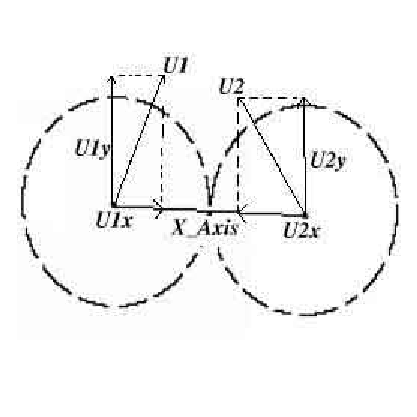
\includegraphics[width=0.35\textwidth]{./img/col.eps}
  \caption{Kolizja bila - bila}
  \label{fig:col}
\end{figure}

Obrazek rzedstawia dwie bile, ich prędkości wektorowe przed zderzeniem, oraz wektory prędkości po zderzeniu rozłożone
na składowe.

\subsection{Prędkość obrotowa, tarcie toczne}

Znając podstawowe wzory fizyczne opisujące prędkość obrotową:

\begin{equation}
\omega = \frac{v}{R}
\end{equation}

obliczaliśmy prędkość obrotową bili na podstawie prędkości liniowej. Ważnym elementem symulacji było 
zamodelowanie tarcia bili przy poruszaniu się po powierzchni stołu bilardowego. Współczynnik tarcia tocznego 
opisany jest zależnością:

\begin{equation}
\mu = \frac{T}{N}R
\end{equation}

Na odstawie tego wzoru obliczyliśmy wartość siły powodującej hamowanie bili podczas ruchu.
\footnote{Wartość współczynnika tarcia jest edytowalna podczas symulacji - można zaobserwować wpływ 
współczynnika na ruch i zachowanie się bil}

\subsection{Kwaterniony jako reprezentacja obrotu}

Na potrzeby projektu należało zaimplementować obsługę operacji na kwarternionach - zwanych nosnikami obrotów.
Było to nieuniknione do prawidłowej reprezentacji obrotów bil.

W skrócie '''postać algebraiczna''' – wprowadzenie oznaczenia dla szczególnych macierzy (kwaternionów):


$i = \left[ \begin{array}{ccc}
i & 0 \\
0 & -i \\
\end{array}
\right]$

$j = \left[ \begin{array}{ccc}
0 & 1 \\
-1 & 0 \\
\end{array}
\right]$

$k = \left[ \begin{array}{ccc}
0 & i \\
i & 0 \\
\end{array}
\right]$

pozwoli na zapis dowolnego kwaternionu w postaci: $q=a+bi+cj+dk$, gdzie $a, b, c, d \in R$.

Po zdefiniowaniu oraz zaimplementowaniu odpowiednich operacji na kwaternionach możliwe było
przeliczanie obrotów w sposób niemal tak łatwy, jak operacje na wektorach przy wyznaczaniu pozycji bili.
